\section{Etude fonctionnelle de l'EPAS}
\subsection{Etude générale}

\begin{figure}[H]
\centering
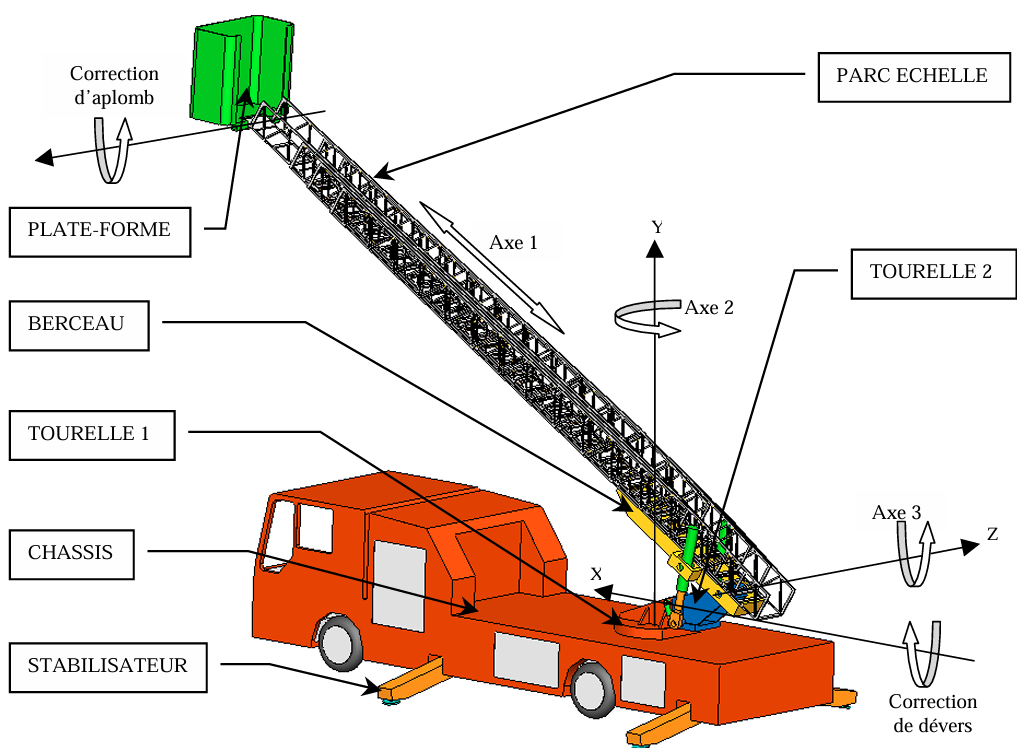
\includegraphics[width=.6\linewidth]{ccinp_psi_2007_fig_02}
\caption{\label{ccinp_psi_2007_fig_02} EPAS}
\end{figure}

Le déplacement de la plate-forme est réalisé suivant trois axes :
\begin{itemize}
\item le déploiement du parc échelle (axe 1) : chaque plan de l’échelle peut se translater par
 rapport aux autres ; seul le quatrième plan d’échelle est solidaire du berceau;
\item le pivotement autour de l’axe Y (axe 2) : la tourelle 1 peut pivoter par rapport au
 châssis autour d’un axe vertical;
\item la rotation autour de l’axe Z (axe 3) : Le berceau peut tourner par rapport à la tourelle
 2 autour d’un axe horizontal.
\end{itemize}

 Pour garantir la sécurité, le système maintient toujours la plate forme en position horizontale :
\begin{itemize}
\item la correction d’aplomb oriente la plate-forme autour d’un axe horizontal parallèle à
 l’axe Z,
\item la correction de devers oriente l’ensemble parc échelle et plate-forme autour de l’axe
 X : la tourelle 2 s’oriente par rapport à la tourelle 1 suivant un axe perpendiculaire aux
 axes 3 et 2.
\end{itemize}
 Lors des déplacements suivant les axes 2 et 3, le système « VARIMAX » de commande des
 actionneurs maintient la vitesse de la plate-forme la plus constante possible afin de limiter les
 mouvements de balancier qui résulteraient d’une commande trop « brusque ».
 
 
Un système de sécurité peut, à tout moment, stopper le déplacement de la plate-forme s’il y a un risque de basculement du camion porteur :
\begin{itemize}
\item des capteurs d’efforts placés sur le parc échelle permettent de tenir compte de la charge dans la
 plate-forme;
\item des capteurs de position sur les trois axes permettent de définir la position de la plate-forme;
\item des capteurs inductifs détectent la position de sortie des stabilisateurs.
\end{itemize}

\question{Complétez le diagramme FAST partiel donné de l’E.P.A.S.}

\subsection{Système de man\oe{}uvre du parc échelle}

 On donne un schéma cinématique du système de manœuvre du parc échelle.

\begin{figure}[H]
\centering
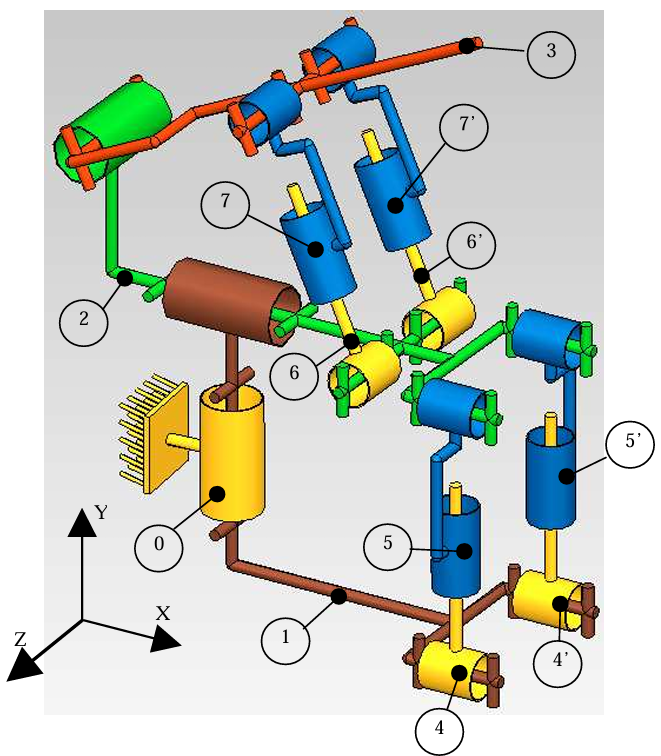
\includegraphics[width=.6\linewidth]{ccinp_psi_2007_fig_03}
\caption{\label{ccinp_psi_2007_fig_03} Schéma cinématique}
\end{figure}


% Q2a
\question{Déterminez le degré d’hyperstatisme de ce mécanisme.}

% Q2b
\question{Proposez des modifications qui permettraient de le rendre isostatique.}


